\documentclass[tikz,border=8pt]{standalone}
\usetikzlibrary{automata,arrows.meta,positioning}
\begin{document}
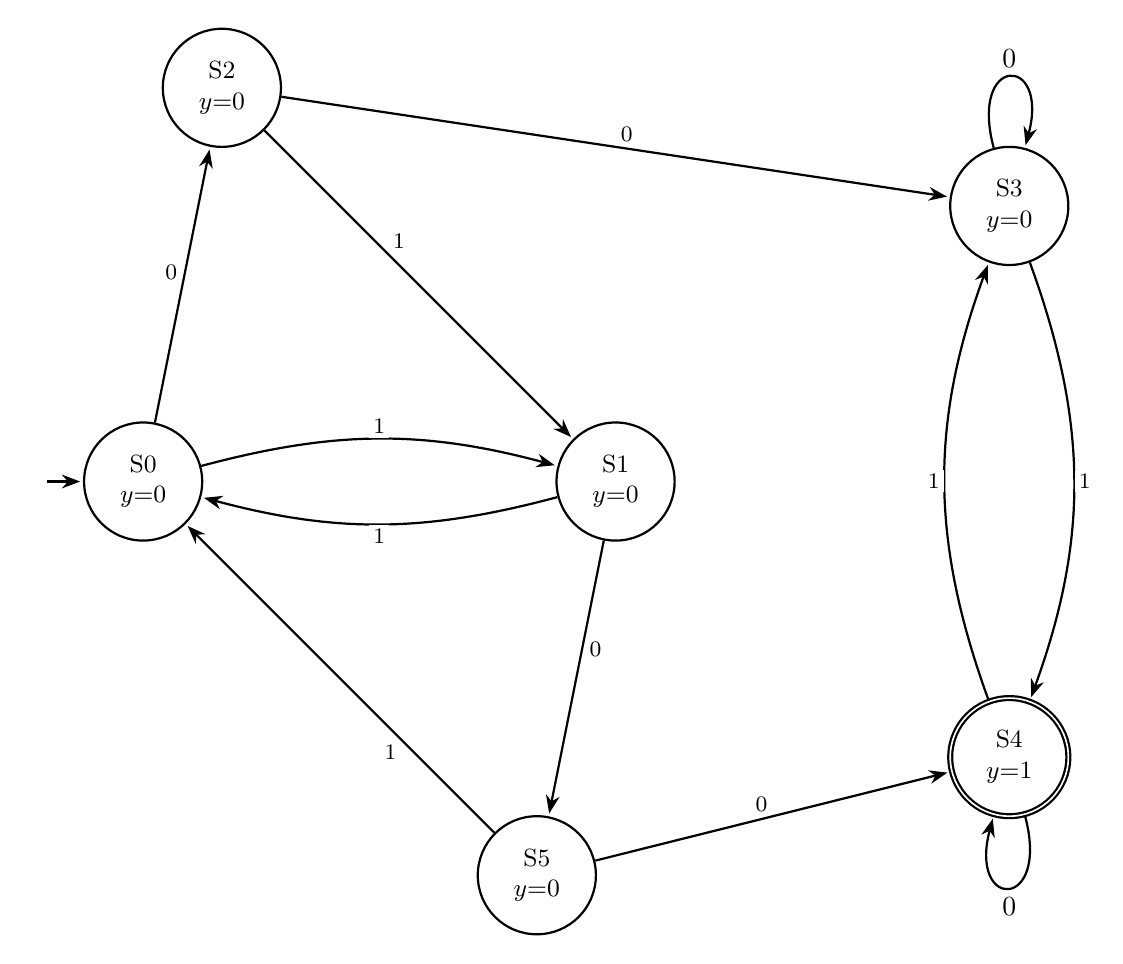
\begin{tikzpicture}[>=Stealth, shorten >=1pt, auto, initial text=, on grid,
  every state/.style={circle,draw,thick,minimum size=1.5cm,inner sep=1pt,font=\small,align=center},
  accepting/.style={accepting by double, accepting distance=2.2pt},
  every edge/.style={draw,thick,->},
  lbl/.style={midway,fill=white,inner sep=1.5pt,font=\footnotesize}]
\node[state,initial] (S0) at (0,0) {S0\\$y{=}0$};
\node[state] (S1) at (6,0) {S1\\$y{=}0$};
\node[state] (S2) at (1,5) {S2\\$y{=}0$};
\node[state] (S5) at (5,-5) {S5\\$y{=}0$};
\node[state] (S3) at (11,3.5) {S3\\$y{=}0$};
\node[state,accepting] (S4) at (11,-3.5) {S4\\$y{=}1$};
\path (S0) edge[bend left=15] node[lbl]{1} (S1)
      (S1) edge[bend left=15] node[lbl]{1} (S0)
      (S0) edge node[lbl]{0} (S2)
      (S2) edge node[lbl,pos=0.4]{1} (S1)
      (S2) edge node[lbl]{0} (S3)
      (S1) edge node[lbl,pos=0.35]{0} (S5)
      (S5) edge node[lbl,pos=0.3]{1} (S0)
      (S5) edge node[lbl]{0} (S4)
      (S3) edge[loop above] node{0} (S3)
      (S3) edge[bend left=20] node[lbl]{1} (S4)
      (S4) edge[bend left=20] node[lbl]{1} (S3)
      (S4) edge[loop below] node{0} (S4);
\end{tikzpicture}
\end{document}
